% !TEX root = UAV_Landing_Pad.tex

\chapter{System  and Unit Testing}

This section describes the approach taken with regard to system and unit testing. 

\section{Overview}
Our testing methodology is based around the following seven areas.

\begin{figure}[tbh]
\begin{center}
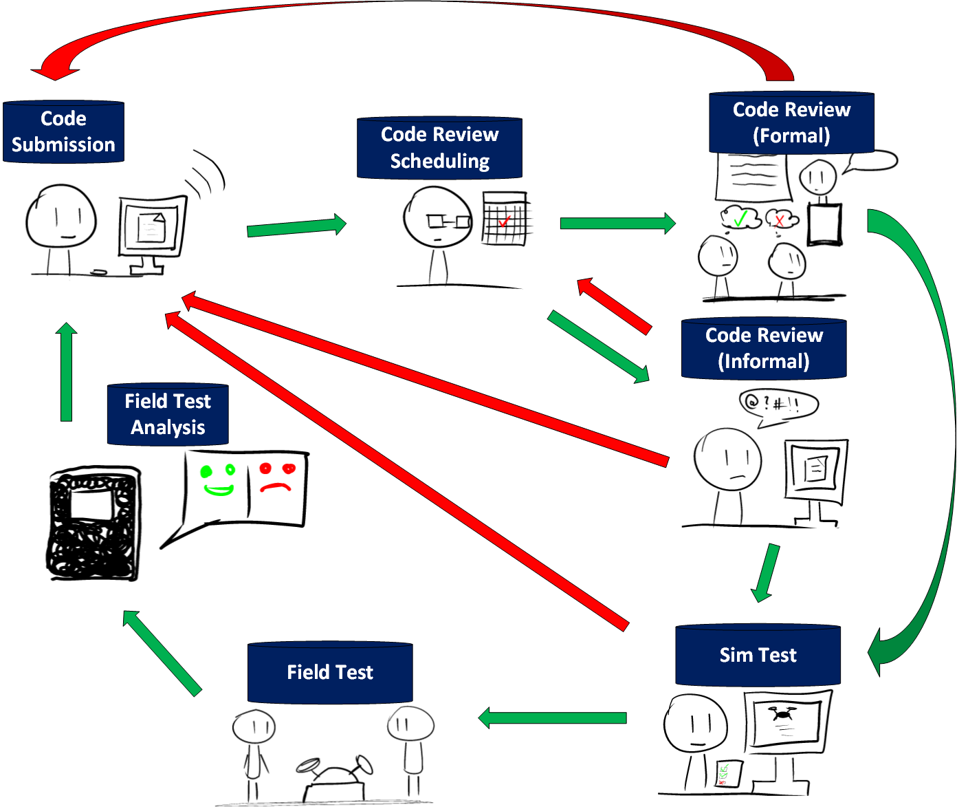
\includegraphics[width=0.6\textwidth]{resources/diagram/Testing}
\end{center}
\caption{Testing Structure \label{systemdiagram}}
\end{figure}

\subsection{Code Submission}
As the development team submits code to the repo, the scrum master will receive an email about the changes. These changes will be based on either the sprint backlog or field test analysis and the changes needed to be made from the results there of.  This change will then trigger code review scheduling.

\begin{figure}[tbh]
\begin{center}

\includegraphics[width=0.6\textwidth]{resources/img/Submission}
\end{center}
\caption{Code Submission \label{systemdiagram}}
\end{figure}


\subsection{Code Review \& Scheduling}

The scrum master will look at the commit logs, filter out documentation and determine what code needs to be scheduled for review.  Either formal (entire team participation) or informal (reviewed soley by a team member or technical lead) reviews will then be scheduled on team member's availibility.  At least two formal reviews will take place during a sprint to provide assurance of quality.  If a code review should fail, the code will be returned and kept from the newest build.


\begin{figure}[tbh]
\begin{center}
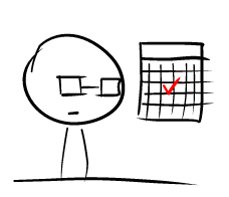
\includegraphics[width=0.6\textwidth]{resources/img/Scheduling}
\end{center}
\caption{Code Review Scheduling \label{systemdiagram}}
\end{figure}


\subsection{Simulation and Field testing}

Upon completion of code review, a Team Member will test the new build on the ROS Simulator, Gazebo.  These tests will determine behavior in current software environment and the newest build will not be added to the physical hardware without passing simulation tests.  This will happen for all code reviews and can be performed as part of a formal code review.  Field testing may not occur immediately after passing simulation testing, however due to scheduling.

During field tests, two team members must be present for documentation purposes.  Reports on the progress of the test will be tracked in lab notebooks or other media and will be uploaded to source control upon completion of the tests.  Problems in software are to be added to the sprint backlog immdediately if not corrected, and resubmitted for code review at this time.  The field testing team members will collaborate with other developers to determine changes for next build.

\begin{figure}[tbh]
\begin{center}

\includegraphics[width=0.6\textwidth]{resources/img/FieldTesting}
\end{center}
\caption{Field Testing \label{systemdiagram}}
\end{figure}

%
%\section{Dependencies}
%FULL SOFTWARE AND HARDWARE LISTS HERE
%
%
%\section{Field Test Reports}
%FIELD TESTS GO HERE

